\section{Anwendungsentwicklung mit Webtechnologien}

Die Sensorverwaltungsanwendung von dryad wird mithilfe von Webtechnologien (html, css, javascript) und zahlreichen Tools entwickelt, um eine Webanwendung zu erstellen, die auf mehreren Plattformen (Browser, ios, Android) läuft und dabei nur einen einzigen Quellcode hat.
Es wurde beschlossen, dass die erste Version der Anwendung eine Single Page Application (SPA) sein sollte.
Derzeit gibt es viele Tools, die das Erstellen einer SPA erleichtern. Innerhalb von Cloud-Team von Dryad wurde beschlossen, die folgenden zu verwenden:

\subsection{Single Page Application (SPA)}

Eine Single Page Application ist ein Website-Design-Ansatz, bei dem der Inhalt jeder neuen Seite nicht durch das Laden neuer HTML-Seiten, sondern dynamisch durch die Fähigkeit von JavaScript, die \ac{DOM}-Elemente auf der bestehenden Seite selbst zu manipulieren, generiert wird.

\begin{figure}[h]
  \centering
  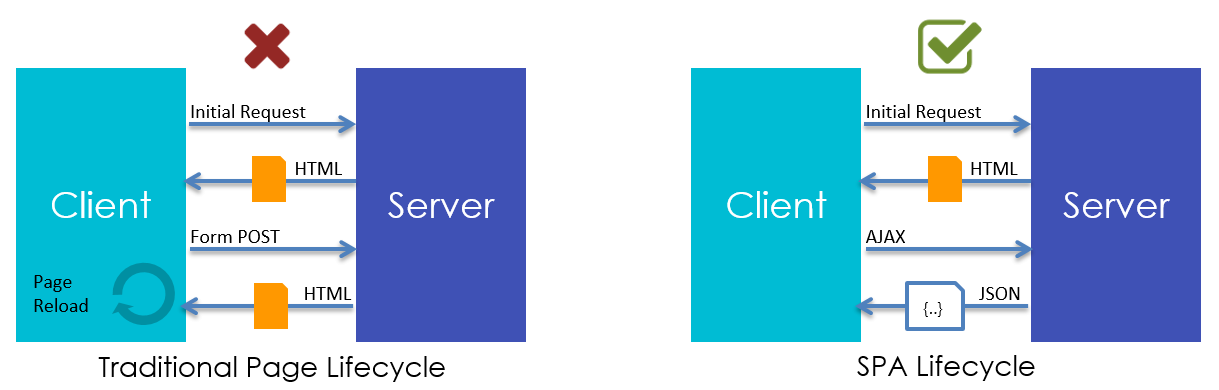
\includegraphics[width=\textwidth]{spa}
  \caption{https://www.tothenew.com/blog/optimization-of-angularjs-single-page-applications-for-web-crawlers/}
  \label{fig:spa}
\end{figure}

\textbf{Pros:}

\begin{itemize}
  \item Die traditionellen HTML-Seiten nehmen beim Hin- und Herbewegen zum Server viel Zeit in Anspruch. Dies erforderte das Nachladen der großen Menge ähnlicher Daten, während das neue SPA die Notwendigkeit der Kommunikation mit HTML-Tags zum Server mildert. SPA lädt nur einmal mit den HTML-Tags, während die nächsten Anfragen auf das teilweise Laden der Seite mittels AJAX und JSON erfolgen. Dies führt zu einer Einsparung von Bandbreite.
  \item Die SPA-Seite wird schneller geladen und benötigt aufgrund der geringeren Datentransaktion weniger Bandbreite. Das Seitendesign und UX werden besser und funktionieren erstaunlich gut mit den langsamen Verbindungen.
\end{itemize}

\textbf{Cons:}

\begin{itemize}
  \item Die traditionellen HTML-Seiten sind gut für den SEO, während die SPA schwer von den Benutzern gecrawlt werden kann, weil die Webcrawler nicht wissen, wie sie mit dem Javascript umgehen sollen. Die Lösung besteht darin, die roboterspezifische HTML-Seite zu kodieren, was wiederum zu Wartungsproblemen führen kann.
  \item Manchmal braucht die SPA viel Zeit, um das Bündel aus CSS und Javascript zu laden, was das erste Laden der Seite verzögert.
\end{itemize}

\subsection{TypeScript}

Die Entwicklung einer Webanwendung kommt heutzutage ohne Javascript kaum noch aus. Die Hegemonie dieser Sprache wird nicht mehr angezweifelt, und ihre Gemeinschaft ist eine der wichtigsten in der Welt der Webentwicklung, was sicherlich auf ihre inhärente Flexibilität zurückzuführen ist. Es hat jedoch einige Einschränkungen, wenn es um die Entwicklung komplexer Anwendungen geht, und aus diesem Grund kommt TypeScript ins Spiel.\cite{tsEssential}

\href{https://www.typescriptlang.org/}{TypeScript}\footnote{https://www.typescriptlang.org/} ist eine Programmiersprache, die von Microsoft im Jahr 2012 entwickelt wurde. Sein Hauptanliegen ist es, die Produktivität der komplexen Anwendungsentwicklung zu verbessern.

Es handelt sich um eine Open-Source-Sprache, die als höhere Schicht von Javascript entwickelt wurde. Jeder in Javascript gültige Code ist auch in TypeScript gültig. Die Sprache führt jedoch optionale Funktionen wie Typisierung oder objektorientierte Programmierung ein. Um diese Funktionen nutzen zu können, ist keine Bibliothek erforderlich, aber nur das Tool für die TypeScript-Kompilierung. Somit wird der ausgeführte Code ein Javascript-Äquivalent des kompilierten TypeScript-Codes sein.

Dieser Sicherheitstyp hat ihn bei Javascript-Entwicklern sehr beliebt gemacht, wie die
\href{https://survey.stackoverflow.co/2022/\#most-loved-dreaded-and-wanted-language-want}{Stackoverflow Survey 2022}\footnote{https://survey.stackoverflow.co/2022/\#most-loved-dreaded-and-wanted-language-want}
beweist:

\begin{figure}[h]
  \centering
  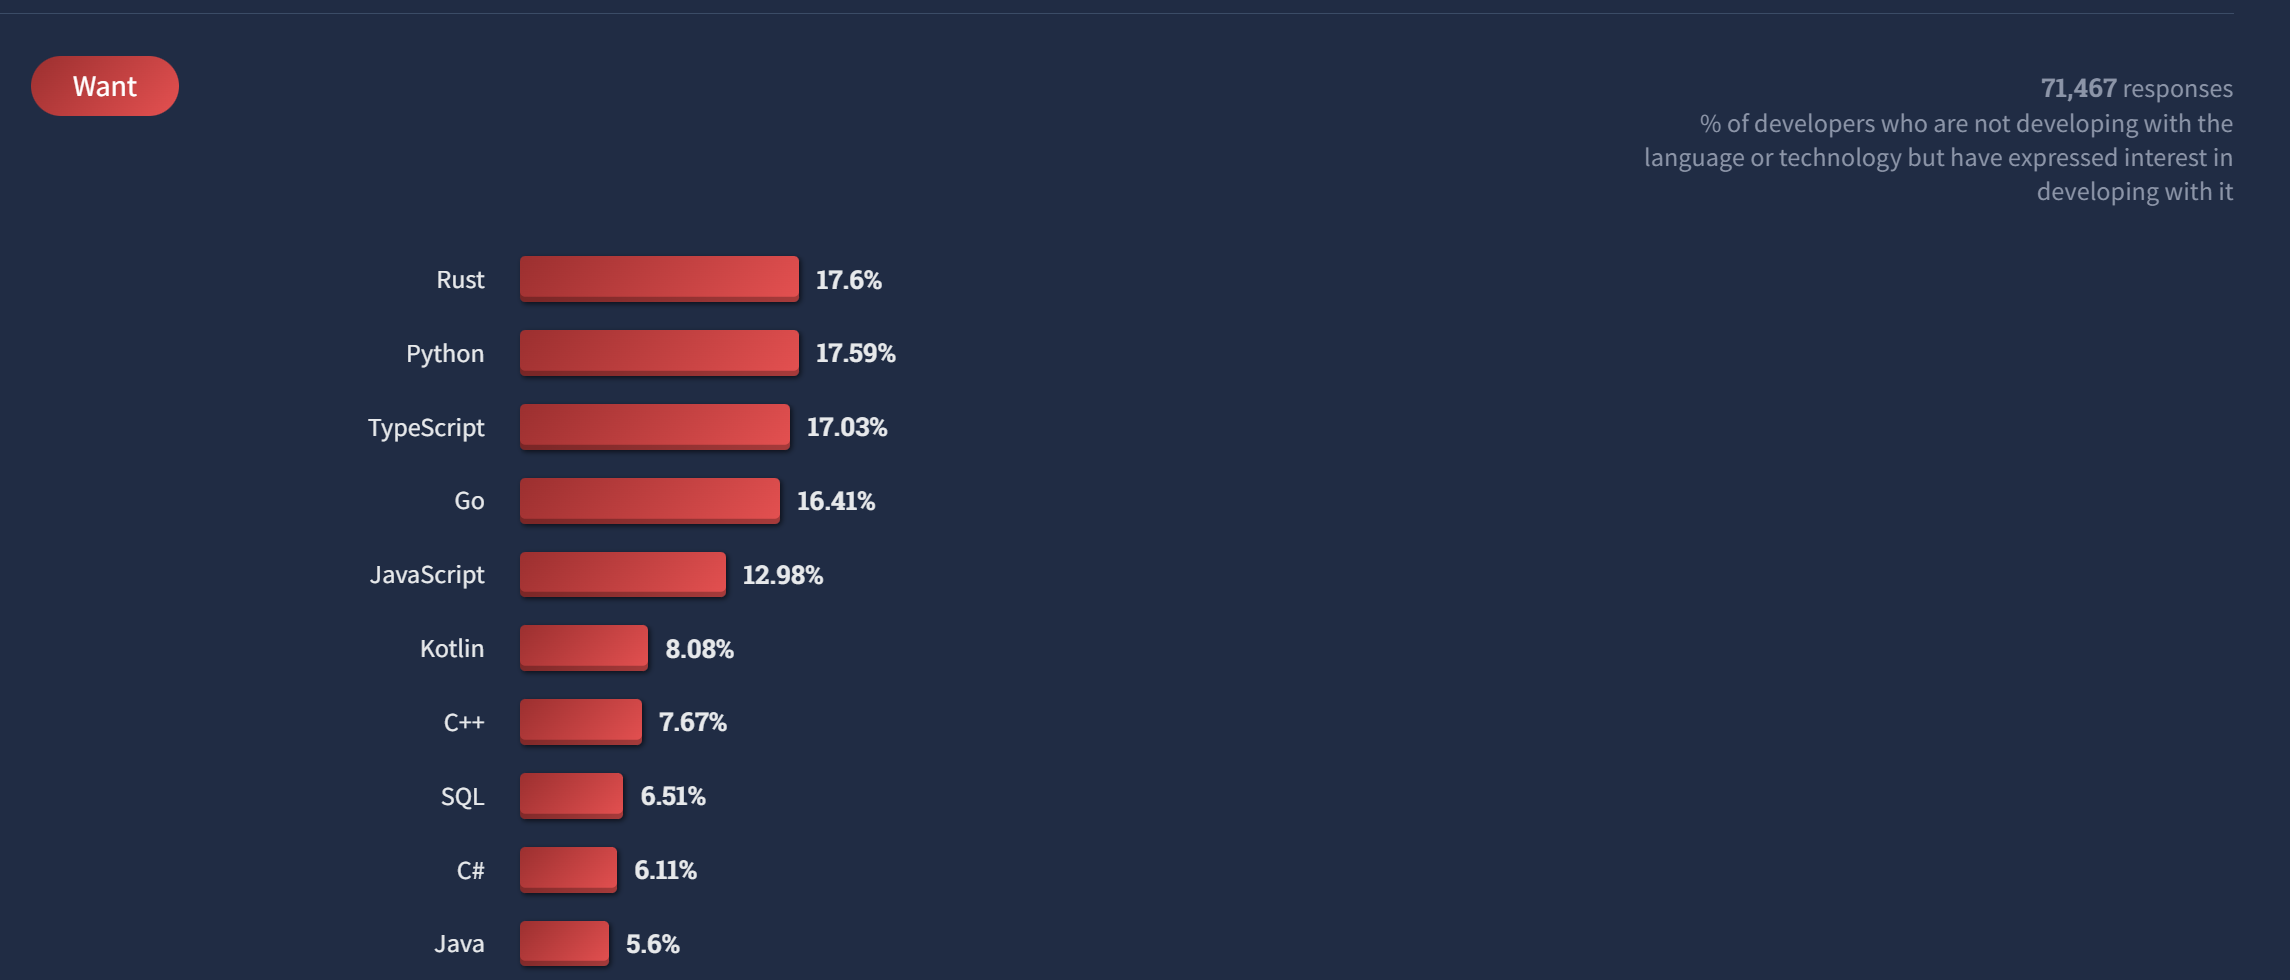
\includegraphics[width=\textwidth]{loved_programming_languages}
  \caption{Liste der beliebtesten Programmier-, Skript- und Auszeichnungssprachen im Jahr 2022}
  \label{fig:spa}
\end{figure}

\subsection{Webpack}
[TODO]
